\documentclass[11pt]{article}

\usepackage[french]{babel}
\usepackage[utf8]{inputenc}
\usepackage{tikz}
\usepackage{pgf}
\usetikzlibrary{arrows,automata}
\usepackage[left=2cm, right=2cm]{geometry}
\usepackage{amsmath}
\usepackage{listings}
\usepackage{graphicx}
\usepackage{multirow}

\date{}
\begin{document}

\def \ETScourse {ELE778-01 - Intelligence artificielle: réseaux neuroniques
et systèmes experts}
\def \ETStitle {Laboratoire 2}
\def \ETSprof  {Cynthia \textsc{Moussa}}
\def \ETSauthA {Liam \textsc{Beguin}\\\emph{BEGL02129304}}
\def \ETSauthB {Louis \textsc{Laporte}\\\emph{LAPL14128903}}
% Author : liambeguin
%
% To use this page add the following in your main page:
%
%\def \ETScourse {ELE430-01 - Conception des filtres Analogiques}
%\def \ETStitle {Laboratoire 2}
%\def \ETSprof {François \textsc{Gourlay}}
%\def \ETSauthA {Liam \textsc{Beguin}\\\emph{BEGL02129304}}
%\def \ETSauthB {Olivier \textsc{Belisle}\\\emph{BELO21098902}}
%\def \ETSauthC {bar}
%% Author : liambeguin
%
% To use this page add the following in your main page:
%
%\def \ETScourse {ELE430-01 - Conception des filtres Analogiques}
%\def \ETStitle {Laboratoire 2}
%\def \ETSprof {François \textsc{Gourlay}}
%\def \ETSauthA {Liam \textsc{Beguin}\\\emph{BEGL02129304}}
%\def \ETSauthB {Olivier \textsc{Belisle}\\\emph{BELO21098902}}
%\def \ETSauthC {bar}
%% Author : liambeguin
%
% To use this page add the following in your main page:
%
%\def \ETScourse {ELE430-01 - Conception des filtres Analogiques}
%\def \ETStitle {Laboratoire 2}
%\def \ETSprof {François \textsc{Gourlay}}
%\def \ETSauthA {Liam \textsc{Beguin}\\\emph{BEGL02129304}}
%\def \ETSauthB {Olivier \textsc{Belisle}\\\emph{BELO21098902}}
%\def \ETSauthC {bar}
%\input{titlepage.tex}

\newcommand{\HRule}{\rule{\linewidth}{0.5mm}}

\begin{titlepage}
	\begin{center}
		\vspace{5cm}
		\textsc{\textbf{\Huge \ETScourse}}
		\vspace{2cm}

		\textsc{\Large \ETStitle }
		\vspace{2.5cm}

		\textsc{\Large Pr\'esent\'e \`a : \\
		\ETSprof}
		\vspace{1.5cm}

		% Bottom of the page
		\vfill
		% Authors
		\begin{minipage}{0.4\textwidth}
			\begin{flushleft}
				\large\ETSauthA
			\end{flushleft}
		\end{minipage}
		\begin{minipage}{0.4\textwidth}
			\begin{flushright}
				\large\ETSauthB
			\end{flushright}
		\end{minipage}
		\begin{minipage}{0.4\textwidth}
			\begin{center}
				\large \ETSauthC
			\end{center}
		\end{minipage}

		\vspace{2cm}
		\HRule \\[0.4cm]
		{ \huge \bfseries \'Ecole de technologie superieure \\[0.4cm] }
		\HRule \\[1.5cm]
		\vspace{1.5cm}

		%date
		{\large \today}
	\end{center}
\end{titlepage}


\newcommand{\HRule}{\rule{\linewidth}{0.5mm}}

\begin{titlepage}
	\begin{center}
		\vspace{5cm}
		\textsc{\textbf{\Huge \ETScourse}}
		\vspace{2cm}

		\textsc{\Large \ETStitle }
		\vspace{2.5cm}

		\textsc{\Large Pr\'esent\'e \`a : \\
		\ETSprof}
		\vspace{1.5cm}

		% Bottom of the page
		\vfill
		% Authors
		\begin{minipage}{0.4\textwidth}
			\begin{flushleft}
				\large\ETSauthA
			\end{flushleft}
		\end{minipage}
		\begin{minipage}{0.4\textwidth}
			\begin{flushright}
				\large\ETSauthB
			\end{flushright}
		\end{minipage}
		\begin{minipage}{0.4\textwidth}
			\begin{center}
				\large \ETSauthC
			\end{center}
		\end{minipage}

		\vspace{2cm}
		\HRule \\[0.4cm]
		{ \huge \bfseries \'Ecole de technologie superieure \\[0.4cm] }
		\HRule \\[1.5cm]
		\vspace{1.5cm}

		%date
		{\large \today}
	\end{center}
\end{titlepage}


\newcommand{\HRule}{\rule{\linewidth}{0.5mm}}

\begin{titlepage}
	\begin{center}
		\vspace{5cm}
		\textsc{\textbf{\Huge \ETScourse}}
		\vspace{2cm}

		\textsc{\Large \ETStitle }
		\vspace{2.5cm}

		\textsc{\Large Pr\'esent\'e \`a : \\
		\ETSprof}
		\vspace{1.5cm}

		% Bottom of the page
		\vfill
		% Authors
		\begin{minipage}{0.4\textwidth}
			\begin{flushleft}
				\large\ETSauthA
			\end{flushleft}
		\end{minipage}
		\begin{minipage}{0.4\textwidth}
			\begin{flushright}
				\large\ETSauthB
			\end{flushright}
		\end{minipage}
		\begin{minipage}{0.4\textwidth}
			\begin{center}
				\large \ETSauthC
			\end{center}
		\end{minipage}

		\vspace{2cm}
		\HRule \\[0.4cm]
		{ \huge \bfseries \'Ecole de technologie superieure \\[0.4cm] }
		\HRule \\[1.5cm]
		\vspace{1.5cm}

		%date
		{\large \today}
	\end{center}
\end{titlepage}



\section{Notations et symboles}
\begin{tabular}{p{1.75cm}p{10cm}}
$\sigma()$ & Fonction d'activation generique \\
\end{tabular}
\newpage



\section{Introduction}
Après avoir fait une étape de pré-traitement lors du laboratoire 2.1, nous
allons maintenant implémenter un reseau de neurones a retro-propagation du
gradient d’erreur dans le but de classifier, le plus précisément possible,
le dataset TiDigits (english spoken digits from 1 to 9).

Pour implémenter ce reseau de neurones, nous utiliserons Python.
Voici une liste d'avantages versus inconvenients qui ont motive notre choix
pour ce language :
\begin{itemize*}
\item avantages:
	\subitem rapidite de developpement
		\subitem lang interprete, pas de compilation
		\subitem modules de calcul matriciel performants
		\subitem language accessible
	\item{inconvenients}
		\subitem lang interprete donc moins rapide \\
\end{itemize*}

Dans un premier temps, nous entrainerons le reseau sur un set de donnees puis
nous evaluerons sa capacite a generaliser sur de nouvelles donnees non utilisees
lors de l'entrainement.

\section{Implementation du r\'eseau de neurones}
\subsection{Architecture globale}
Comme dit en introduction, Nous allons implementer un reseau de neurones a
retro-propagation du gradient d'erreur. Ici, nous enoncerons les notations et
equations 'generiques' utilisees au sein du reseau.

l'ensemble des calculs sont effectues sous forme matricielle afin de simplifier
et generaliser les equations mais aussi de mieux tirer avantage des ressources
des ordinateurs utilises.

\paragraph{Feedforward:} cette etape propage l'entree a travers l'ensemble du
reseau et enregistre toutes les variables intermediaires.
\begin{equation}
	\begin{aligned}
		{\bf z}_x^{(l)} &=  {\bf w}^{(l)} \cdot {\bf a}_x^{(l-1)} + {\bf b}^{(l)}\\
		{\bf a}_x^{(l)} &=  \sigma({\bf z}_x^{(l)})\\
	\end{aligned}
\end{equation}
Pour avoir la prediction finale du reseau ${\bf \hat{y}}$, il faut repeter l'etape
ci-dessus pour chaque couche. Pour la derniere couche, on obtient:
\begin{equation}
	\begin{aligned}
		{\bf z}_x^{(L)} &=  {\bf w}^{(L)} \cdot {\bf a}_x^{(L-1)} + {\bf b}^{(L)}\\
		{\bf \hat{y}}_x &=  \sigma({\bf z}_x^{(L)})\\
	\end{aligned}
\end{equation}

\paragraph{La fonction de cout}est la fonction utilisee lors du processus
d'entrainement pour evaluer l'erreur entre la prediction du reseau
${\bf \hat{y}}$ et la sortie attendue ${\bf y}$. Les differents fonctions
disponibles seront detaillees dans une prochaine section.
Pour la suite, nous l'appelerons de fa\c con generique: $C({\bf w}, {\bf b})$.

\paragraph{retro-propagation:} Cette \'etape calcule l'impacte de chaque poids
(et seuil) sur l'erreur finale. Pour obtenir l'erreur $\delta_j^l$ due au neurone
$j$ de la couche $l$, il faut propager l'erreur de la sortie vers l'entree
avec les equations suivantes:

\begin{equation}
	\begin{aligned}
		{\boldsymbol \delta}^L &= \frac{\partial C}{\partial {\bf z}^L} =
		\frac{\partial C}{\partial {\bf a}^L} \circ \frac{\partial {\bf a}^L}{\partial {\bf z}^L} \\
		&= \frac{\partial C}{\partial {\bf a}^L} \circ \sigma'({\bf z}^L)
		= \frac{\partial C}{\partial {\bf \hat y}} \circ \sigma'({\bf z}^L)\\
		&= C'({\bf w}, {\bf b}) \circ \sigma'({\bf z}^L)\\
	\end{aligned}
\end{equation}

De la m\^eme mani\`ere, on definit une notation recursive:
\begin{equation}
	\begin{aligned}
		{\boldsymbol \delta}^l &= \frac{\partial C}{\partial {\bf z}^l} =
		\frac{\partial C}{\partial {\bf z}^{(l+1)}} \circ
		\frac{\partial {\bf z}^{(l+1)}}{\partial {\bf z}^l} \\
		&= \boldsymbol \delta^{(l+1)} \circ \frac{\partial {\bf z}^{(l+1)}}{\partial {\bf z}^l} \\
	\end{aligned}
\end{equation}

Or,
\begin{equation}
	\begin{aligned}
		\frac{\partial {\bf z}^{(l+1)}}{\partial {\bf z}^l} &= \\
	\end{aligned}
\end{equation}

Etant donne que le r\'eseau doit \^etre tr\`es flexible quant au nombre de
couches et au nombre de neurones, nous utiliserons un tuple pour instancier
notre r\'eseau.
Chaque \'el\'ement de la liste repr\'esente une couche du r\'eseau
(incluant la couche d'entr\'ee) et sa valeur d\'etermine le nombre de neurones
present sur la couche.

D'autre part, on nous demande aussi que le reseau soit capable d'utiliser
differentes fonctions d'activation. Base sur cette contrainte, nous avons
choisi d'aussi donner a l'utilisateur la possibilite de choisir entre differentes
fonctions de cout et differentes fonctions de regularization.

\subsection{Extraction des donn\'ees}
% TODO
% preprocessing, chx du 40, 50 ,60
% normalisation du dataset
% classification homme / femme


\subsection{Initialisation du res\'eau}
Lorsque le reseau est instanci\'e, les parametres tels que $\eta$ et $\lambda$
sont copi\'es dans l'object
\emph{Network} et les matrices de poids et de seuils (\emph{weights} et
\emph{biases}) sont g\'en\'er\'ees. Les dimensions de ces matrices sont
determin\'ees en fonction du nombre de neurones sur chaque couche et du nombre
de couches $L$ \`a l'aide de la methode suivante:

Soit, $w_{ij}^{(l)}$ le poid connectant le neurone $i$ de la couche $(l-1)$ au
neurone $j$ de la couche $(l)$. \\
O\`u :
\begin{equation}
	\left \{
	\begin{aligned}
		&1 \le l \le L \\
		&0 \le i \le d^{(l-1)} \\
		&1 \le j \le d^{(l)} \\
	\end{aligned}
	\right .
\end{equation}
On definit donc ${\bf w}^{(l)}$ la matrice de dimension $((l) \times (l-1))$
connectant la couche $(l-1)$ \`a la couche $(l)$ cr\'eant ainsi, $(L-1)$ matrices
de poids sur l'ensemble du reseau. \\

D'autre part, du fait que la fonction aleatoire utilis\'ee pour l'initialisation
des poids donne une distribution avec les parametres suivants $\mu=0$ et $\sigma=1$,
l'initialisation des poids a tendance a saturer les neurones et ralentire l'apprentissage.
car :
\begin{equation}
	\begin{aligned}
		Var(z) &= \sum_{i=1}^N(Var(x_i)) \\
		Var(z) &= N \cdot Var(x) \\
		\sigma(z) &= \sqrt{N} \cdot 1 \\
		\sigma(z) &= \sqrt{N}
	\end{aligned}
\end{equation}




\begin{figure}[htp]
	\centering
	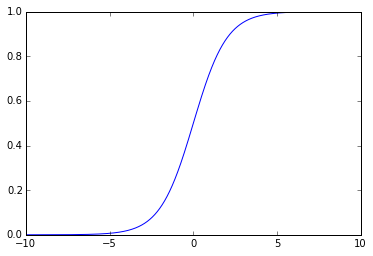
\includegraphics[scale=.5]{img/sigmoid_sat.png}
	\caption{Visualisation de la saturation de la fonction \emph{sigmoid} si
	$|z| \ge 5$.}
\end{figure} \\

Pour contrer cette saturation et donc accelerer les premi\`eres \'epoques
d'apprentissage, nous utiliserons une distribution plus \'etroite avec les
parametres $\mu=0$ et $\sigma =1/\sqrt{N}$ \\


\lstset{tabsize = 4,
frame=lines,
numbers=left,
captionpos=b,
caption = {Initialisation des poids et seuils},
language = python,
basicstyle=\small} \\
\begin{lstlisting}
self.biases  = [ np.random.randn(y, 1) for y in struct[1:] ]
self.weights = [ np.random.randn(y, x) / np.sqrt(x) \
				for x, y in zip(struct[:-1], struct[1:]) ]
\end{lstlisting}


\subsection{Fonctions d'activation}
% sigmoid  -> probability dist
% tanh     -> soft threshold (linear arround 0 hard threshold far)
% softplus -> linear above 0
% add plots



\subsection{Fonctions de cout}
% cross-entropy -> prevent neuron saturation
Comme ennonce precedemment, nous offrons aussi \`a l'utilisateur la possibilite
de choisir parmis differentes fonctions de couts, la fonctions que le reseau
cherche a minimiser en ajustant les poids et seuils des connections.
\paragraph{quadratic}

\subsection{Eviter le sur-apprentisage}
% plus ya de neurons plus on peut overfit -> polynome a plus de dimensions
\subsubsection{Early stopping}
% add this image https://upload.wikimedia.org/wikipedia/commons/thumb/1/1f/Overfitting_svg.svg/1024px-Overfitting_svg.svg.png?1469206069861
\subsubsection{Validation crois\'ee}
% leave one out, K folds, implique de 'bouger' des trucs dans les datasets
% merge train et VC -> larger traiing set
\subsubsection{Fonctions de r\'egularisation}
% penalise le poids large check :
% http://neuralnetworksanddeeplearning.com/chap3.html#overfitting_and_regularization

\subsection{Entrainement}
% batch gradient descent
% stochastic gradient descent
% minibatch GD check network.py

\subsection{Ajustement des hyper-param\`etres}
% http://neuralnetworksanddeeplearning.com/chap3.html#how_to_choose_a_neural_network's_hyper-parameters

\subsection{Inspection du res\'eau}

\section{Interface graphique}



\section{Discussions}
\subsection{Problemes rencontr\'es}
\subsection{Methodes de r\'esolution}
\subsection{conclusion et possibilites d'amelioration}
% ajouter autres pistes d'amelioration
% conclure sur performance globale du systeme
% classification homme/femme

\end{document}
% vim: cc=80 :
